\documentclass[a4paper,12pt]{article}
\usepackage[left=2cm, right=2cm, top=2cm]{geometry}
\usepackage{graphicx} 
\usepackage[export]{adjustbox}
\usepackage{titlepic}
\usepackage{amssymb}
\usepackage{titling}
\usepackage[utf8]{inputenc}
\usepackage{listings}
\usepackage{color}
\usepackage[T1]{fontenc}
\usepackage[utf8]{inputenc}
\usepackage{wrapfig}
\usepackage{helvet}
\usepackage{fourier} 
\usepackage{array}
\usepackage{makecell}
%\usepackage[square,sort,comma,numbers]{natbib}
\usepackage{ragged2e}
\usepackage{placeins}
\bibliographystyle{IEEEtran}
\usepackage{float}
\setlength{\belowcaptionskip}{-15pt}
\renewcommand{\familydefault}{\sfdefault}
\newcommand{\squeezeup}{\vspace{-2.5mm}}
\definecolor{codegreen}{rgb}{0,0.6,0}
\definecolor{codegray}{rgb}{0.5,0.5,0.5}
\definecolor{codepurple}{rgb}{0.58,0,0.82}
\definecolor{backcolour}{rgb}{0.95,0.95,0.92}

\renewcommand\theadalign{bc}
\renewcommand\theadfont{\bfseries}
\renewcommand\theadgape{\Gape[4pt]}
\renewcommand\cellgape{\Gape[4pt]}

\usepackage{fancyhdr,lipsum}
\pagestyle{fancy}
\fancyhf{}% Clear header/footer

\usepackage{hyperref}
\hypersetup{
    colorlinks,
    %citecolor=gray,
    citecolor=black,
    filecolor=black,
    linkcolor=black,
    urlcolor=black,
    linktoc=all
}

\lstdefinestyle{mystyle}{
    backgroundcolor=\color{backcolour},   
    commentstyle=\color{codegreen},
    keywordstyle=\color{blue},
    numberstyle=\tiny\color{codegray},
    stringstyle=\color{codepurple},
    basicstyle=\tiny,
    breakatwhitespace=false,         
    breaklines=true,                 
    captionpos=b,                    
    keepspaces=true,                 
    numbers=left,                    
    numbersep=5pt,                  
    showspaces=false,                
    showstringspaces=false,
    showtabs=false,                  
    tabsize=2
}


\chead{%
  \ifcase\value{page}
  % empty test for page = 0
  \or % page=1
  \or % page = 2
  \or Alexander Bolton% page = 3
  \or Alexander Bolton% page = 4
  \or Alexander Bolton% page = 5
  \or Alexander Bolton% page = 6
  \or Alexander Bolton% page = 7
  \or Sam Wilcock% page = 8
  \or Sam Wilcock% page = 9
  \or Sam Wilcock% page = 10
  \or Sam Wilcock% page = 11
  \or John Jakobsen% page = 12
  \or John Jakobsen% page = 13
  \or John Jakobsen% page = 14
  \or John Jakobsen% page = 15
  \or Conclusion Author% page = 16
  \or Author% page = 13
  \or % page = 14
  \else
  % Empty chead here!
  \fi
}

\cfoot{\thepage}

\lstset{style=mystyle}

\pretitle{%
  \begin{center}
  \LARGE
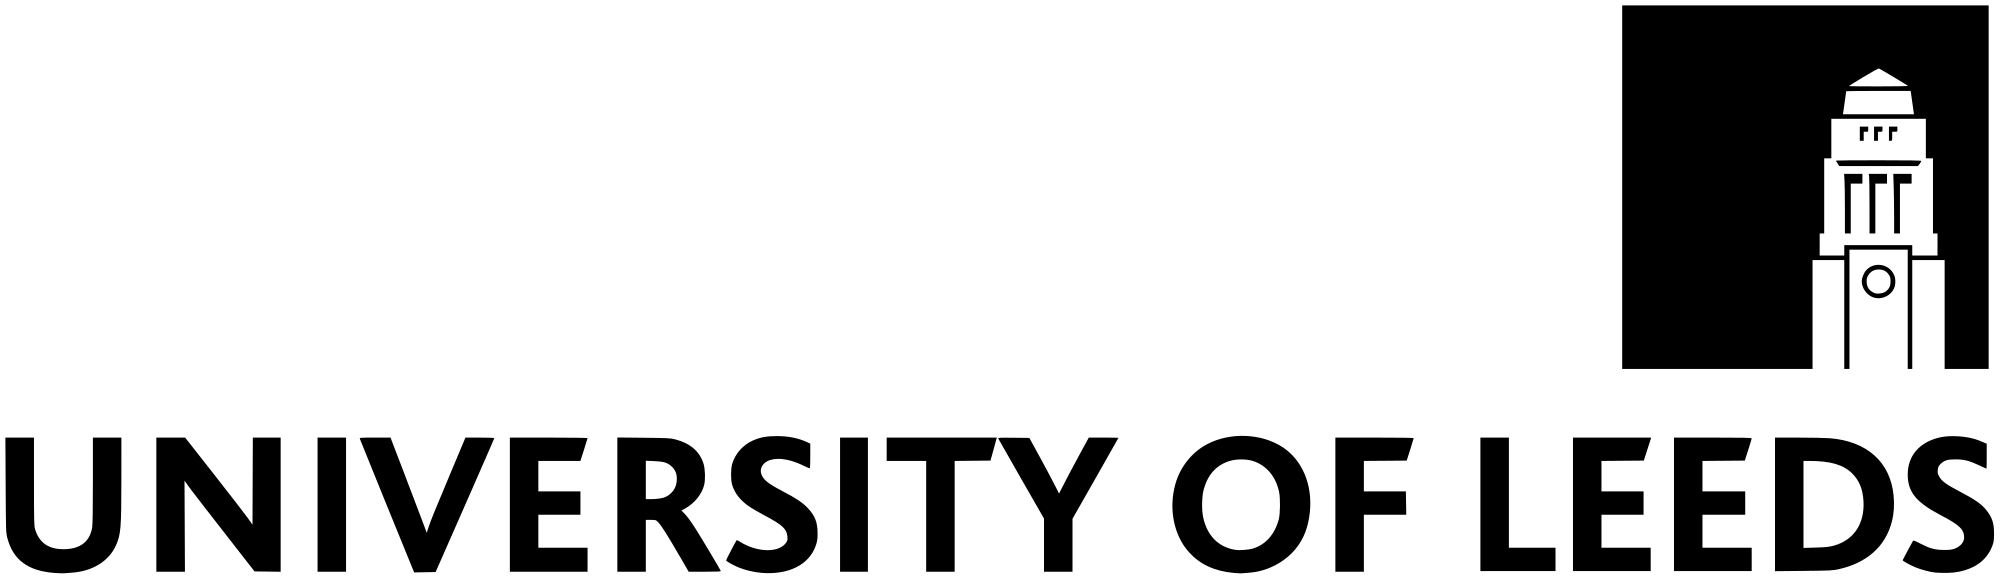
\includegraphics[width=0.5\textwidth, right]{UniLogo.png}\\[\bigskipamount]

\hspace{15cm}

\hspace{27cm}

\hspace{27cm}

\hspace{10cm}
}
\posttitle{\end{center}}	

\begin{document}

\title{\\ \textbf{ELEC5620M \\ Mini Project \\ \- \\ DE1-SoC Pong }}
\author{Alexander Bolton - 200938078 \\ Sam Wilcock - 201285260\\ John Jakobsen - }
\date{May 2019}
\maketitle
\begin{center}
Submitted in accordance with the requirements for the degree of \\
Master of Science in Embedded Systems Engineering
\end{center}
\vfill
\begin{center}
The University of Leeds \\  School of Electronic and Electrical Engineering
\end{center}
\newpage

\tableofcontents
\newpage 
\section{Introduction}
\begin{flushleft}
This report will discuss the group project for the Embedded Microprocessor System Design module. The groups member's were Alexander Bolton, Sam Wilcock, and John Jakobsen. The projects aim was to create a game of Pong on the DE1-SoC's microprocessor unit (MPU) which utilised the LT24 LCD Screen, a VGA screen, PS2 keyboard controls, button controls, and have audio output.
\\ \- \\
This report will be broken down into sections with section 1 being the introduction. Section 2 will discuss the display and graphics side of the project including the VGA driver which controls the monitor, the display driver which controls both LCD and VGA screens with a frame buffer, sprites and text which will go into depth of how the sprites are created, finally game engine graphics which will go into how the game engine uses the sprites including destroying, creating, and moving the sprites. 
\\ \- \\
Section 3 will discuss...
\\ \- \\
Section 4 will discuss...
\\ \- \\
Section 5 will be the conclusion which will summarise the report and discuss if we have met the aims of the project. It will discuss what could be improved upon and changed. All code will be placed in the end of the report in the appendices. 
\end{flushleft}
\newpage
\section{Display and Graphics}
\subsection{VGA Driver}
\begin{flushleft}
This subsection discusses the VGA driver and how it was implemented in the project. The VGA video out supports 640x480 however in this project is set to the default value of 320x240 pixels. The image displays from the VGA controller which is addressed from a pixel buffer. Each pixel value is write addressable using equation 1. An example of the pixel at 0,1 is shown in equation 2. The default base address for the pixel buffer is 0xC8000000 as stated in the manual. \cite{altera_2014} 
\begin{equation}
	VGA_{base address} + (pixelX_{coordinates}\:pixelY_{coordinates}\:0_{2})
\end{equation}
\begin{equation}
	C8000000_{16} + (00000001\:000000000\:0)_{2} = C8000400_{16}
\end{equation}
The pixels are layed out with the y coordinate starting from the top to bottom of the screen. The x coordinate is from right to left of the screen as shown in figure 1.
\begin{figure}[H]
	\centering
	\fbox{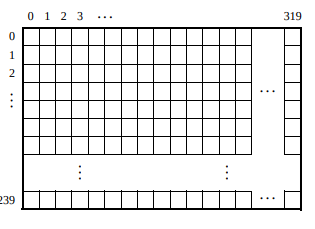
\includegraphics[width=0.4\textwidth]{./images/VGAPixels.png}}
	\caption{Pixel layout for pixel buffer of VGA controller \cite{altera_2014}}
\end{figure}
\- \\
Each pixel once addressed can be set to a value of colour with by setting bits for red, green, and blue. Each colour is allocated 5 bits which indicate the strength of colour for the pixel as shown in figure 2. 
\begin{figure}[H]
	\centering
	\fbox{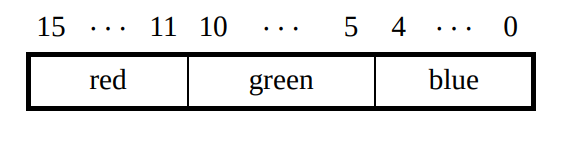
\includegraphics[width=0.3\textwidth]{./images/VGAPixelcolour.png}}
	\caption{Pixel Colour Layout \cite{altera_2014}}
\end{figure}
\- \\
This code extracted from the project shows how a pixel is set in C.
\begin{figure}[H]
	\centering
	\lstinputlisting[language=C, firstline=20, lastline=25, frame=bt]{../DE1_SOC_PONG/DE1SoC_VGA/DE1SoC_VGA.c}
		\caption{Code used to set pixel to a colour.}
\end{figure}
\end{flushleft}
\newpage
\subsection{Display Driver}
\begin{flushleft}
This subsection discusses the display driver which allows pixels to be set to a frame buffer and refreshed on command. The frame buffer is made up of 2 types of arrays which were a front frame buffer (what's currently on screen) and a rear frame buffer (what wants to be put onto the screen). The advantage of this is that it allows pixels to be checked and allows refresh on command. 
\\ \- \\
 Once the screen is desired to be refreshed the memory is compared between the front frame buffer and rear frame buffer to check if they are the same. If not the frame buffers are updated by checking each pixel in the frame buffers values. Any differences then update to display and to the front frame buffer. When first creating this frame buffer a problem with articulating occurred which is believed due to a memory overflow. The decision was made to split the frame buffer into 2 halves which reduced the memory used in each array which alleviated the issue. \\ \- \\
Checking the pixels in a frame buffer is a very slow process so multiple frame buffers were created to experiment with. This experimentation involved splitting the screen into multiple sections and finding how many sections would be the fastest. This improved performance as multiple frame buffers were checked in memory and making the changes was done by comparing all pixels in a smaller area when there was a change in that area. In this experimentation frame buffers of 1 section to 8 sections were created. It was found that the 8 section frame buffer yielded the faster rendering of the frame buffer to the screens. All frame buffers were kept in the library which can be set. As it was still a slow process for the game a frame skip feature was also added to which skips a number of frames before refreshing. This speeds up the game dramatically. Also added to reduce errors and prevent system crashing was a 'Displays\_setWindow' when set this prevents the driver from trying to address pixels outside of the window.
\\ \- \\
To compare frame buffers quickly the function 'memcmp' was used which set a variable in the function. If a change was found then the frame buffer would update.
\begin{figure}[H]
	\centering
	\lstinputlisting[language=C, firstline=443, lastline=455, frame=bt]{../DE1_SOC_PONG/pongDisplay/pongDisplay.c}
		\caption{Code used to compare and update the buffers (Quad buffer)}
\end{figure}
\- \\
A number of function were created for use by the engine. These are functions such as 'Displays\_init' which initialises the displays, 'Displays\_mode' to set which buffer to use, 'Displays\_setPixel' to set the pixel to a colour in rear buffer, 'Displays\_Refresh' to refresh the buffer to hardware, 'Displays\_ForceRefresh' to force a display refresh regardless of frame skip count, and finally 'Displays\_getPixel' which returns the value of the colour of the pixel requested.
\end{flushleft}
\newpage
\subsection{Sprites and Text}
\begin{flushleft}
This subsection discusses how sprites are rendered and created in the library and how text is also created. There are 2 main sprites for this game of pong.
\\ \- \\
The first sprite is the ball. The ball must be initialised into an array before it can be rendered. To initialise the ball Pythagoras theorem was used (as previously completed in the graphics library of a previous assessment in this module). Equation 3 is Pythagoras theorem equation which is used. When the result is equal to or is less than radius squared then the value in the array is set to 1. The code iterates from the centre point for all values of x and y and sets an array. This was created as such to allow the ball to be dynamically set in size. Once rendered the ball can be rendered by providing coordinates of where to render (from centre of ball) and a colour. This will use these values and set the pixels to the frame buffer.
\begin{equation}
	Radius^{2} = x^{2} + y^{2}
\end{equation}
\begin{figure}[H]
	\centering
	\fbox{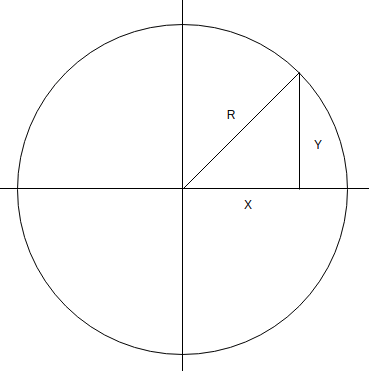
\includegraphics[width=0.3\textwidth]{./images/PyCir.png}}
	\caption{Pythagoras Theorem demonstrated inside circle}
\end{figure}
\- \\
The paddle was set by iterating through a square of defined values and setting pixels to the colour desired by iterating through the height and width of the rectangle and setting values to the desired colour.
\\ \- \\
When generating and rendering text a library of hex values is used. The user inputs the character array of text they wish to use. These hex values are at 90 degree angles so the code first rotates the text 90 degrees to be upright for each letter in the char array into a letter array. A for loop is then used to set the pixels of the letter array to the frame buffer. If small then the is simply reads from the letter array and sets the appropriate pixel. If large 1 pixel in the letter array sets 4 pixels in the frame buffer. This allows large bold text. 
\end{flushleft}
\newpage
\subsection{Game Engine Graphics}
\begin{flushleft}
•
\end{flushleft}
\newpage
\section{Controls and Menus}
\newpage
\section{Game Physics}
\newpage
\section{Conclusion}
\begin{flushleft}

\end{flushleft}
\newpage
\section{Appendix}
\newpage
\addcontentsline{toc}{section}{References}
\begin{flushleft}
\bibliography{refs}
\end{flushleft}
\end{document}
